 \documentclass{article}
    \usepackage{amsmath}
    \usepackage[utf8]{inputenc}
    \usepackage[english]{babel}
    \usepackage{color}
    \usepackage{graphicx}
    \usepackage{enumitem}
    \usepackage{incgraph}
    \hyphenpenalty=10000
    \exhyphenpenalty=10000
    % \usepackage[T1]{fontenc}
    % \usepackage{geometry}
    \usepackage[top = 2cm, bottom = 2cm]{geometry}
    
    \usepackage[familydefault,light]{Chivo} 
    \usepackage[T1]{fontenc}
    
    \setlength{\parindent}{4em}
    \setlength{\parskip}{2em}
\renewcommand{\baselinestretch}{1.5}
    \usepackage{graphicx}
    
    \usepackage{listings}
    \usepackage{color}
    
    \definecolor{dkgreen}{rgb}{0,0.6,0}
    \definecolor{gray}{rgb}{0.5,0.5,0.5}
    \definecolor{mauve}{rgb}{0.58,0,0.82}
    
    \lstset{frame=tb,
      language=ocaml,
      aboveskip=3mm,
      belowskip=3mm,
      showstringspaces=false,
      columns=flexible,
      basicstyle={\small\ttfamily},
      numbers=none,
      numberstyle=\tiny\color{gray},
      keywordstyle=\color{blue},
      commentstyle=\color{dkgreen},
      stringstyle=\color{mauve},
      breaklines=true,
      breakatwhitespace=true,
      tabsize=3
    }
    
    \title{COL 783 \\ Assignment 5}
    \author{Rajbir Malik \\ 2017CS10416}
    
    \begin{document}
    
    \maketitle

%  Starting page
% -------------------------------------------------------
% -------------------------------------------------------
    \begin{center}
    \Large{\underline{\textbf{Texture Synthesis}}}
    \end{center}
    \subsection*{Overview}
    We were tasked with implementing algorithms which are used in generic texture generation. It was an exciting assignment, where we came across various methods, set on different principles and progressive improvements.\\
    We used random phase shifting to try out changes in frequency and thus random edge shifts.\\
    We also tried matching pyramids of random noises with original templates getting the desired textures from the noise.\\
    Also, finally, we took the rigid, brute method for neighbourhood matching and texture generation. We exploited the fact that textures are locally repetitive.
% -------------------------------------------------------
% -------------------------------------------------------
% Topic I
    \pagebreak
    \subsection*{Random phase noise}
% -------------------------------------------------------
    The simplest approach is based on Fourier descriptors, i.e. the amplitudes of the Fourier coefficients of the image. Creating a random image with the same descriptors is equivalent to retaining the Fourier amplitudes while randomizing their phases.\\
\textbf{Results}\\
    The random phase noise generation of textures, led to promising textures when working with broadly uniform unstructured textures, changing whose phase would only lead to another distribution of the same pattern.\\
    Whenever some structure, even minimal, was observed the texture generated drifted significantly from the original texture.\\
    Results are presented below...\\
% -------------------------------------------------------
    \begin{figure}[!htb]
    %
    \minipage{0.5\textwidth}
    \begin{center}
      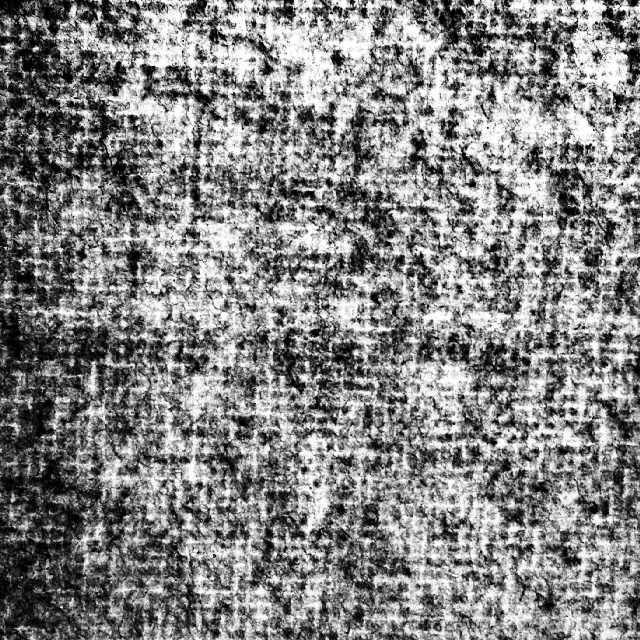
\includegraphics[scale=.3]{5/report/random/6.png}
      \caption{Original}
    \end{center}
    \endminipage \hfill
    %
    \minipage{0.5\textwidth}
    \begin{center}
      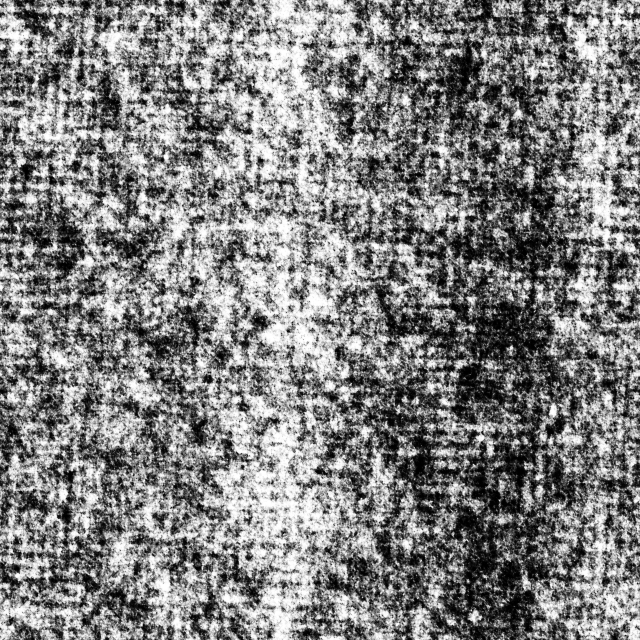
\includegraphics[scale=.3]{5/report/random/6_c.png}
      \caption{Generated}
    \end{center}
    \endminipage
    %
    \end{figure}

% -------------------------------------------------------
\pagebreak
    \begin{figure}[!htb]
    %
    \minipage{0.5\textwidth}
    \begin{center}
      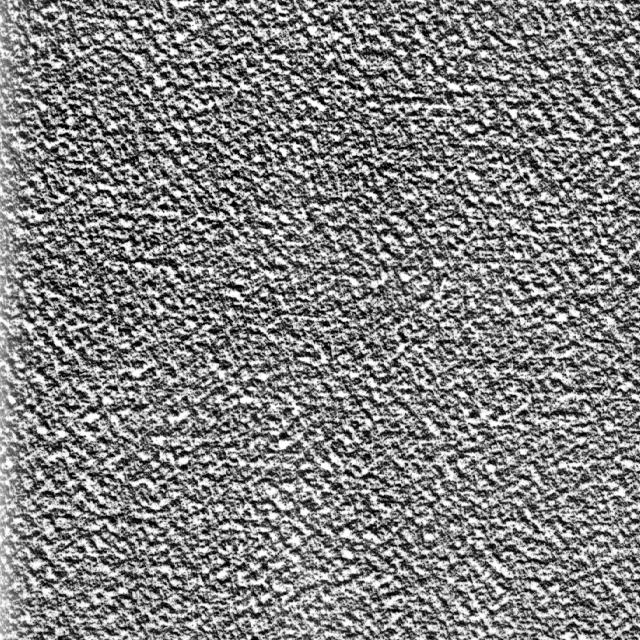
\includegraphics[scale=.3]{5/report/random/7.png}
      \caption{Original}
    \end{center}
    \endminipage \hfill
    %
    \minipage{0.5\textwidth}
    \begin{center}
      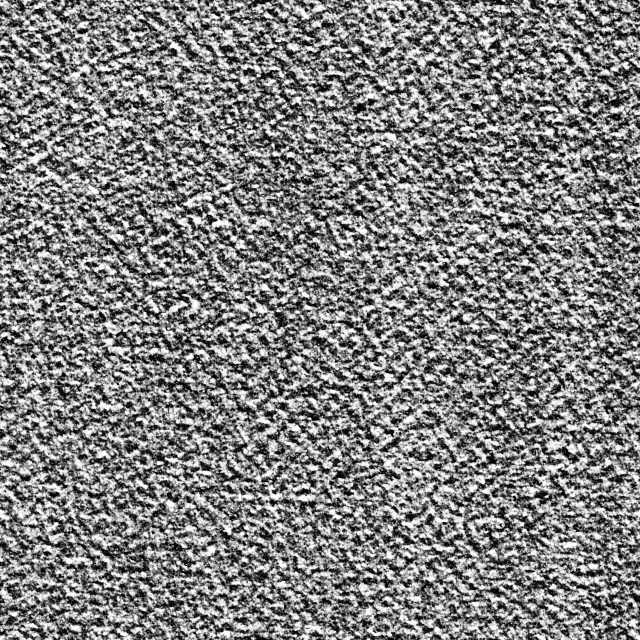
\includegraphics[scale=.3]{5/report/random/7_c.png}
      \caption{Generated}
    \end{center}
    \endminipage
    %
    \end{figure}
    
    \begin{figure}[!htb]
    %
    \minipage{0.5\textwidth}
    \begin{center}
      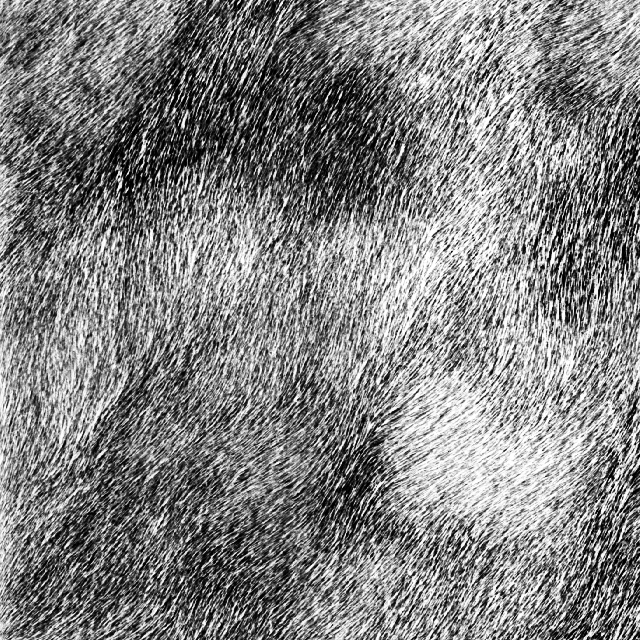
\includegraphics[scale=.3]{5/report/random/8.png}
      \caption{Original}
    \end{center}
    \endminipage \hfill
    %
    \minipage{0.5\textwidth}
    \begin{center}
      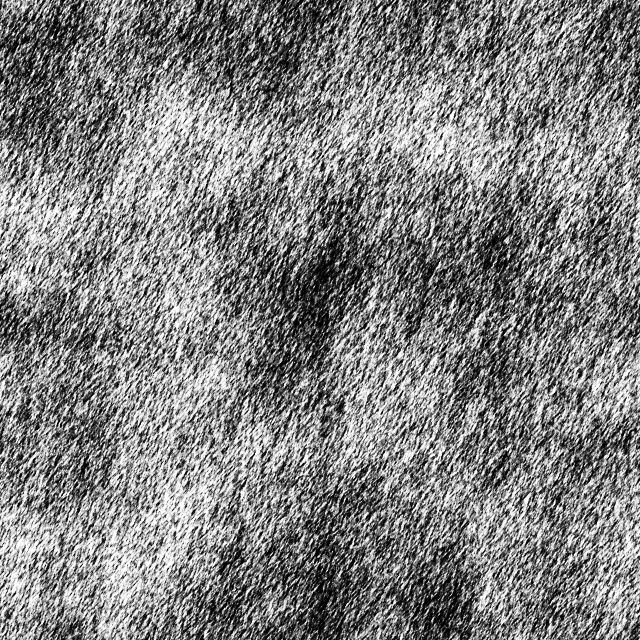
\includegraphics[scale=.3]{5/report/random/8_c.png}
      \caption{Generated}
    \end{center}
    \endminipage
    %
    \end{figure}

    
    It is observable that the examples laid lack certain structure.\\[5pt]
    Also, since, all the examples so far are monochrome there isn't a need to consider the channel interdependence.
    
% -------------------------------------------------------
\pagebreak

    \begin{figure}[!htb]
    %
    \minipage{0.5\textwidth}
    \begin{center}
      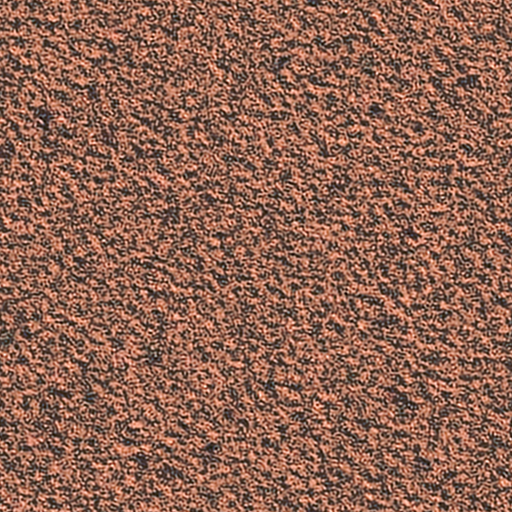
\includegraphics[scale=.4]{5/report/random/1.png}
      \caption{Original}
    \end{center}
    \endminipage \hfill
    %
    \minipage{0.5\textwidth}
    \begin{center}
      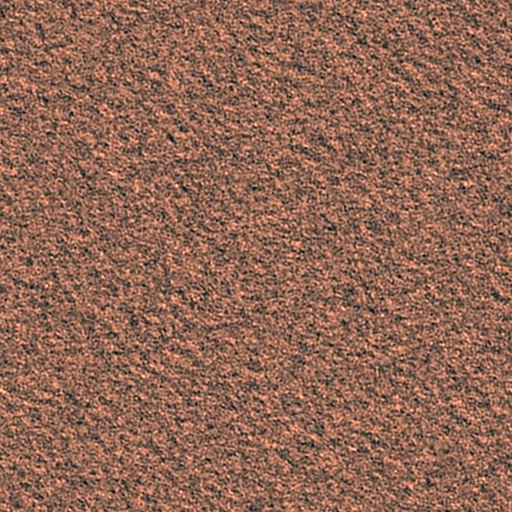
\includegraphics[scale=.4]{5/report/random/1_c.png}
      \caption{Generated}
    \end{center}
    \endminipage
    %
    \end{figure}
    
    \begin{figure}[!htb]
    %
    \minipage{0.5\textwidth}
    \begin{center}
      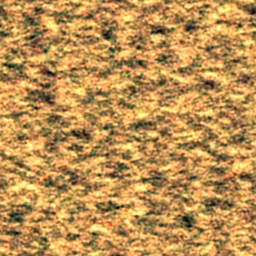
\includegraphics[scale=0.8]{5/report/random/2.png}
      \caption{Original}
    \end{center}
    \endminipage \hfill
    %
    \minipage{0.5\textwidth}
    \begin{center}
      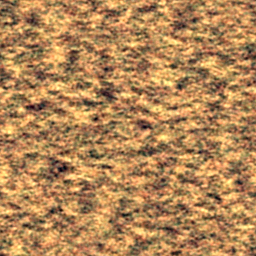
\includegraphics[scale=0.8]{5/report/random/2_c.png}
      \caption{Generated}
    \end{center}
    \endminipage
    %
    \end{figure}

    It is observable that the examples above too, lack certain structure. But there is substantial color-based dependence/correlation.\\[5pt]
    Now, to maintain such relation while randomising the frequency content, what can be done is converting the image to \textbf{YUV} channel (which supports color-independence across channels).

% -------------------------------------------------------
\pagebreak
There are multitude of cases where RPN fails to derive the desired results, mostly these arise due to constrained and structured features in the texture which are destroyed by the randomisation.\\ Few are presented below...\\[10pt]

    \begin{figure}[!htb]
    %
    \minipage{0.5\textwidth}
    \begin{center}
      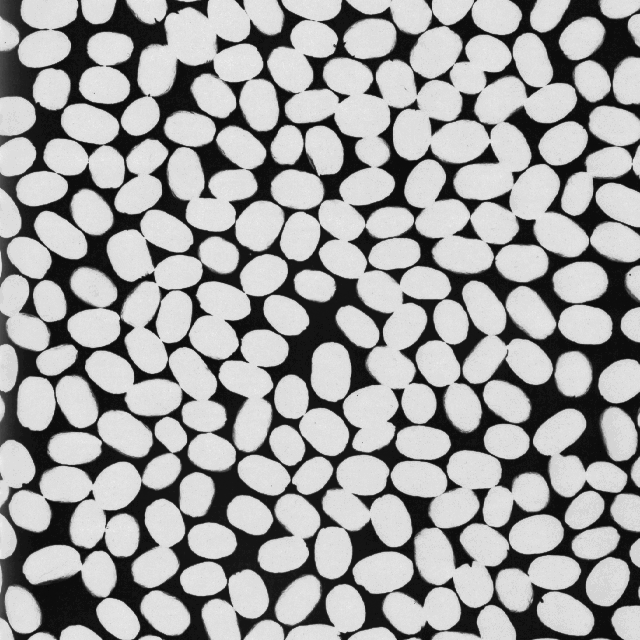
\includegraphics[scale=.3]{5/report/random/3.png}
      \caption{Original}
    \end{center}
    \endminipage \hfill
    %
    \minipage{0.5\textwidth}
    \begin{center}
      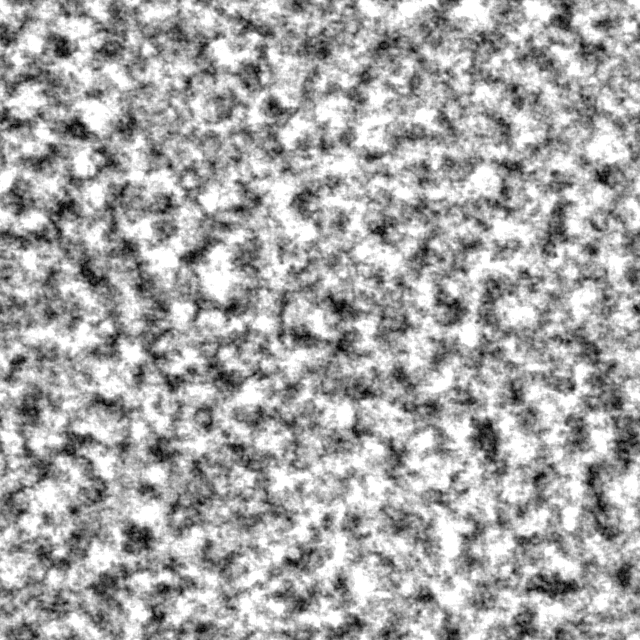
\includegraphics[scale=.3]{5/report/random/3_c.png}
      \caption{Generated}
    \end{center}
    \endminipage
    %
    \end{figure}
    
    \begin{figure}[!htb]
    %
    \minipage{0.5\textwidth}
    \begin{center}
      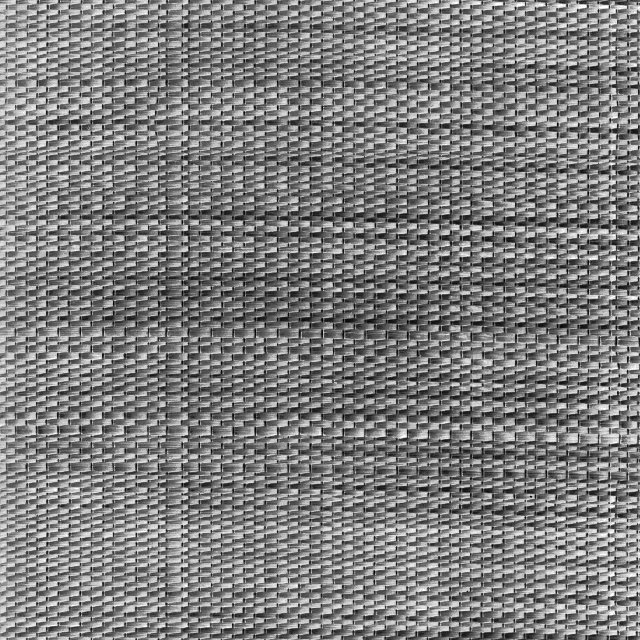
\includegraphics[scale=.3]{5/report/random/4.png}
      \caption{Original}
    \end{center}
    \endminipage \hfill
    %
    \minipage{0.5\textwidth}
    \begin{center}
      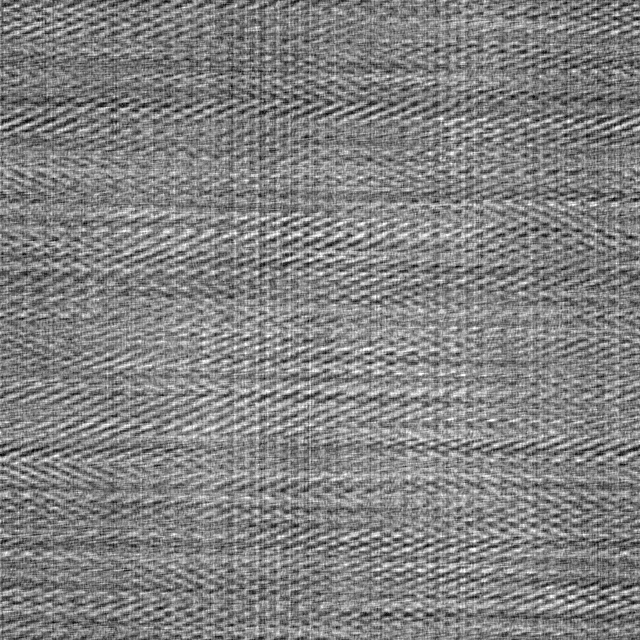
\includegraphics[scale=.3]{5/report/random/4_c.png}
      \caption{Generated}
    \end{center}
    \endminipage
    %
    \end{figure}
% -------------------------------------------------------
\pagebreak

    \begin{figure}[!htb]
    %
    \minipage{0.5\textwidth}
    \begin{center}
      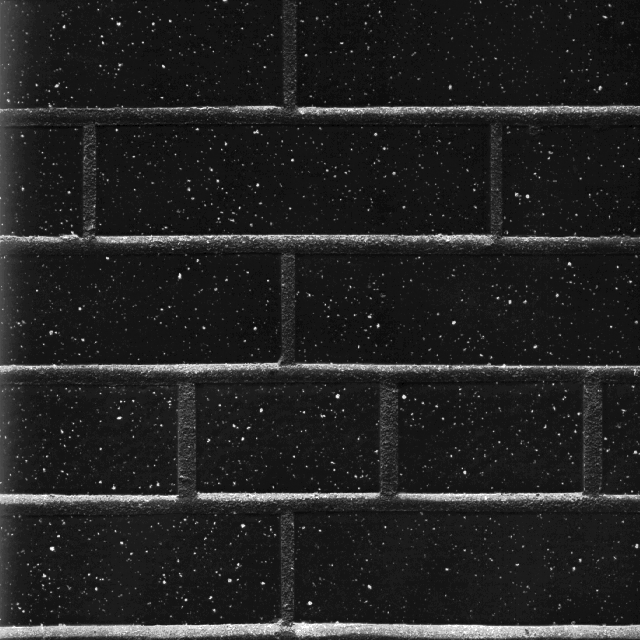
\includegraphics[scale=.3]{5/report/random/5.png}
      \caption{Original}
    \end{center}
    \endminipage \hfill
    %
    \minipage{0.5\textwidth}
    \begin{center}
      
\includegraphics[scale=.3]{5/report/random/5_c.png}
      \caption{Generated}
    \end{center}
    \endminipage
    %
    \end{figure}

    \begin{figure}[!htb]
    %
    \minipage{0.5\textwidth}
    \begin{center}
      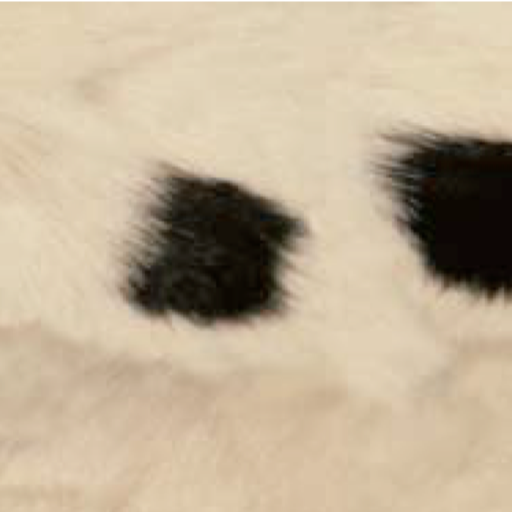
\includegraphics[scale=.35]{5/report/random/11.png}
      \caption{Original}
    \end{center}
    \endminipage \hfill
    %
    \minipage{0.5\textwidth}
    \begin{center}
      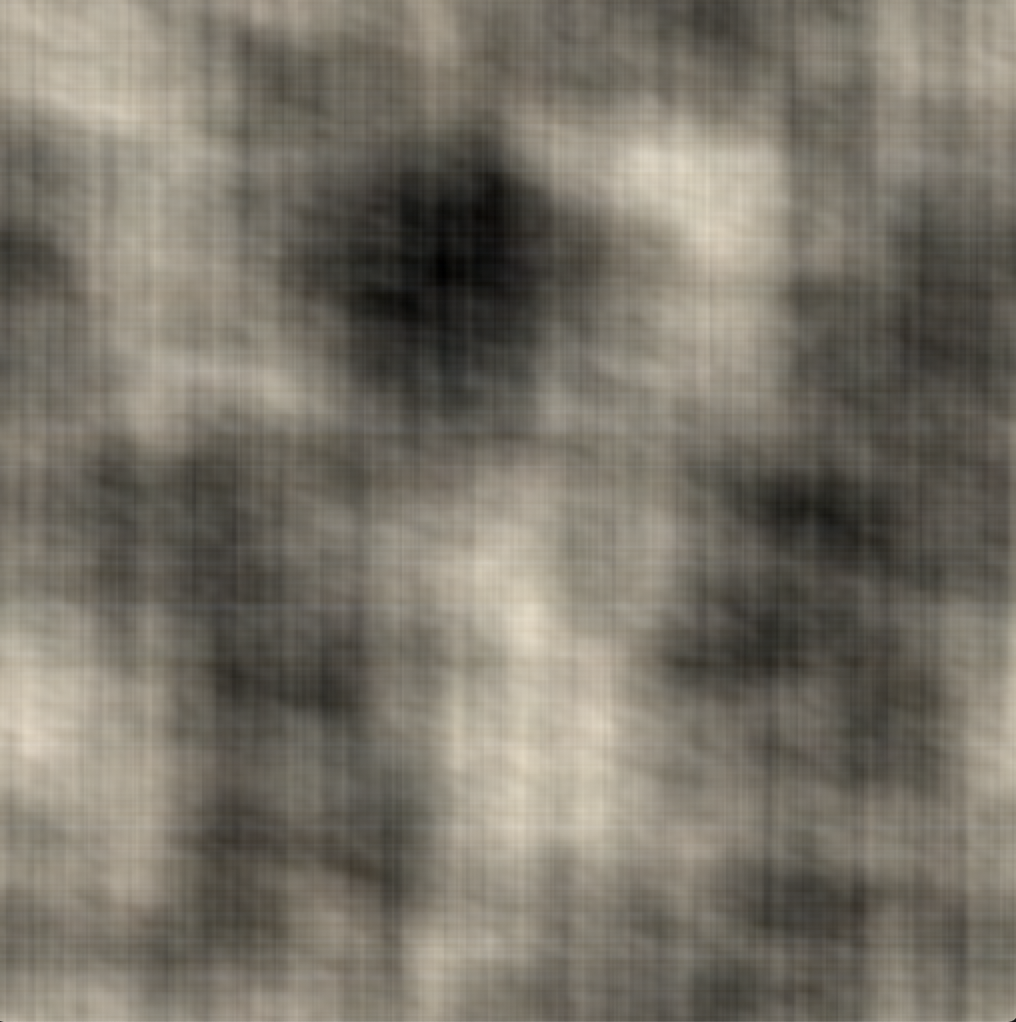
\includegraphics[scale=.35]{5/report/random/11_c.png}
      \caption{Generated}
    \end{center}
    \endminipage
    %
    \end{figure}    

    \begin{figure}[!htb]
    %
    \minipage{0.5\textwidth}
    \begin{center}
      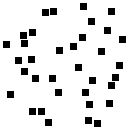
\includegraphics[scale=1.2]{5/report/random/9.png}
      \caption{Original}
    \end{center}
    \endminipage \hfill
    %
    \minipage{0.5\textwidth}
    \begin{center}
      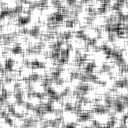
\includegraphics[scale=1.2]{5/report/random/9_c.png}
      \caption{Generated}
    \end{center}
    \endminipage
    %
    \end{figure}

% -------------------------------------------------------
% -------------------------------------------------------
% Topic I
    \pagebreak
    \subsection*{Steerable Pyramids}
% -------------------------------------------------------
    Here, starting with gaussian white noise, I was able to reduce them to textures by mapping there steerable pyramids successively till a decent convergence was observed.\\
    The basic motivation is that the steerable pyramids are able to carve out all texture features separately and map them to noise features by histogram matching.\\
    One of the most important things to take care of, while using steerable pyramids on colored images, is to decorrelate the color bands such that the random noise doesn't perturb histogram matching and thus giving vague colorings. This has been shown below...\\
% -------------------------------------------------------
    
    \begin{figure}[!htb]
    \minipage{\textwidth}
    \begin{center}
        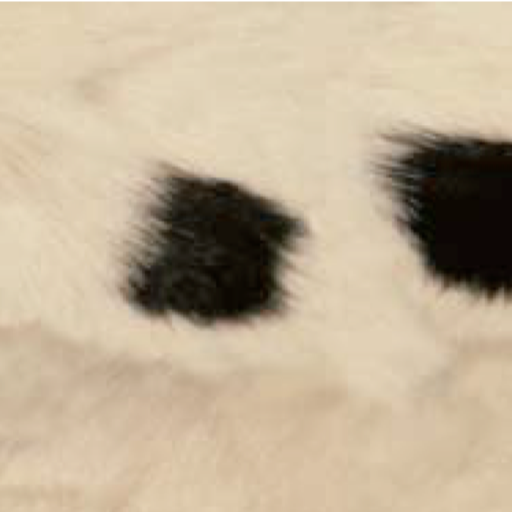
\includegraphics[scale=.25]{5/report/steerable/6.png}
      \caption{Image}
    \end{center}
    \endminipage \hfill
    \end{figure}

    \begin{figure}[!htb]
    %
    \minipage{0.5\textwidth}
    \begin{center}
      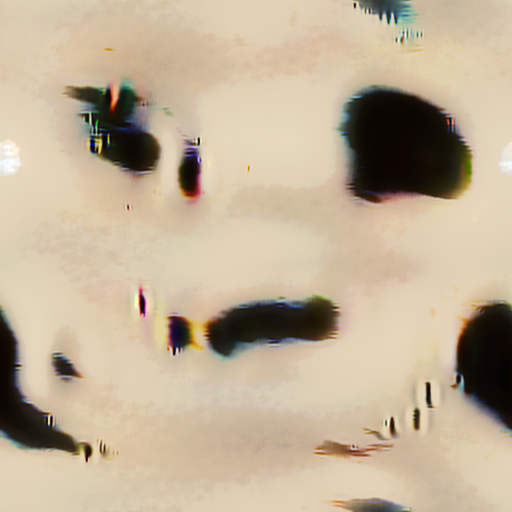
\includegraphics[scale=.35]{5/report/steerable/6_c_u2.png}
      \caption{Generated (No Decorrelation)}
    \end{center}
    \endminipage \hfill
    %
    \minipage{0.5\textwidth}
    \begin{center}
      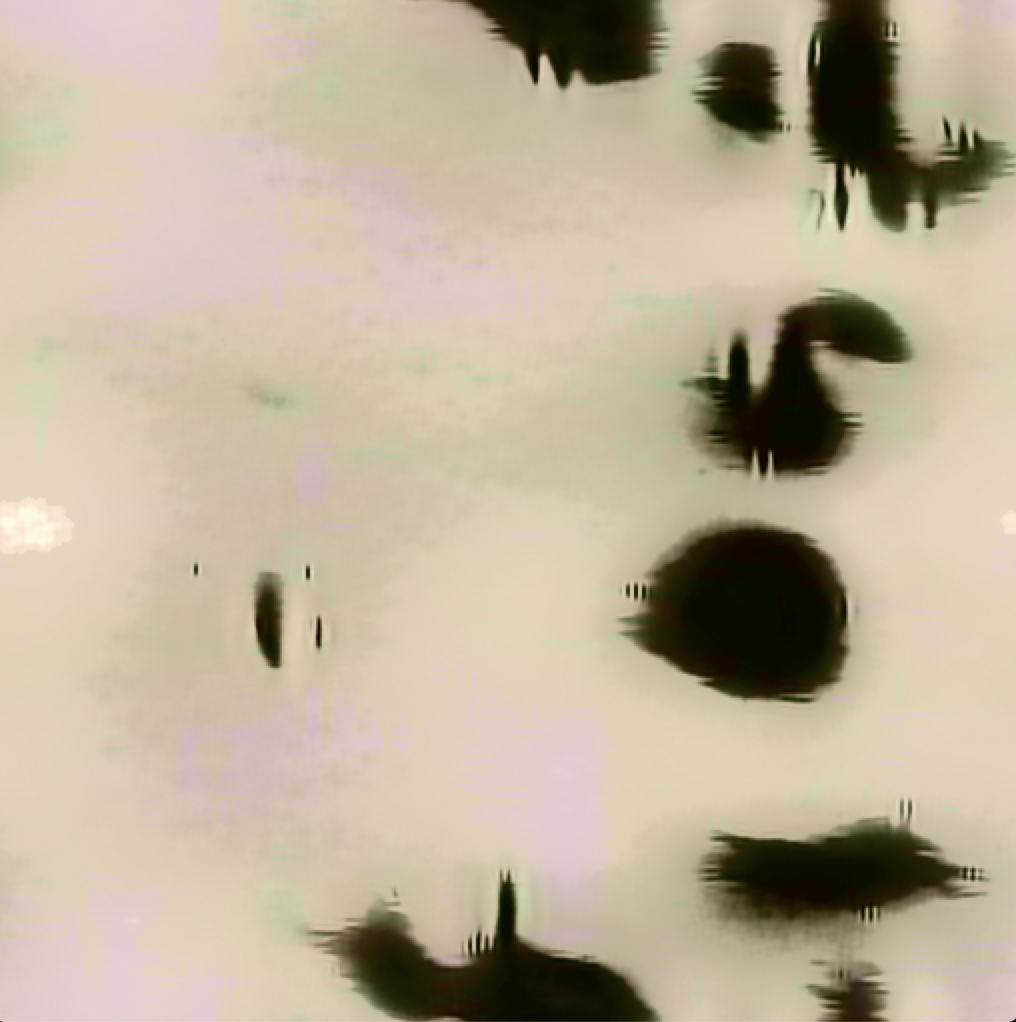
\includegraphics[scale=.35]{5/report/steerable/6_c2.png}
      \caption{Generated (Decorrelation)}
    \end{center}
    \endminipage
    %
    \end{figure} 
% -------------------------------------------------------
\pagebreak\\
Keeping the above formulation in mind, the results are presented below...\\

    \begin{figure}[!htb]
    %
    \minipage{0.5\textwidth}
    \begin{center}
      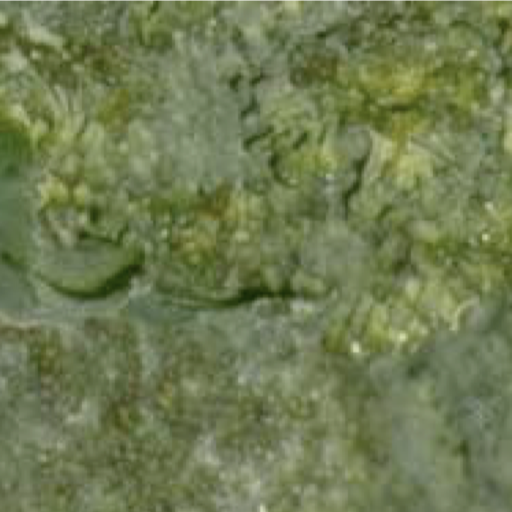
\includegraphics[scale=.32]{5/report/steerable/1.png}
      \caption{Original}
    \end{center}
    \endminipage \hfill
    %
    \minipage{0.5\textwidth}
    \begin{center}
      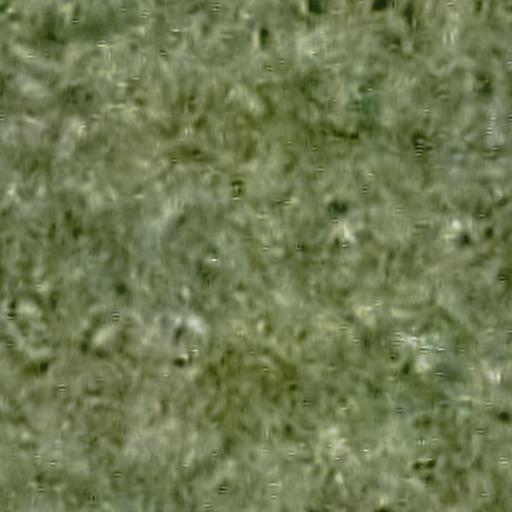
\includegraphics[scale=.32]{5/report/steerable/1_c.png}
      \caption{Generated}
    \end{center}
    \endminipage
    %
    \end{figure} 

    \begin{figure}[!htb]
    %
    \minipage{0.5\textwidth}
    \begin{center}
      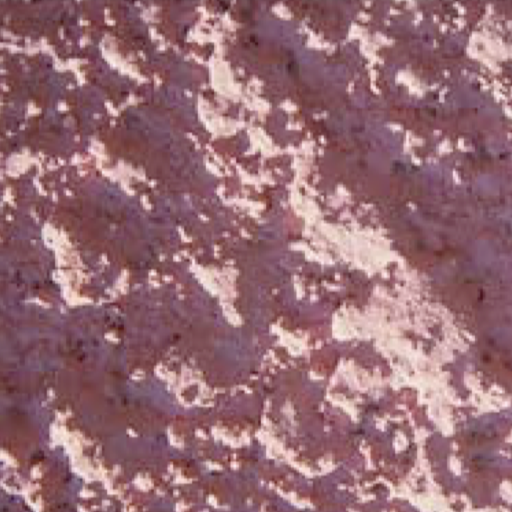
\includegraphics[scale=.32]{5/report/steerable/2.png}
      \caption{Original}
    \end{center}
    \endminipage \hfill
    %
    \minipage{0.5\textwidth}
    \begin{center}
      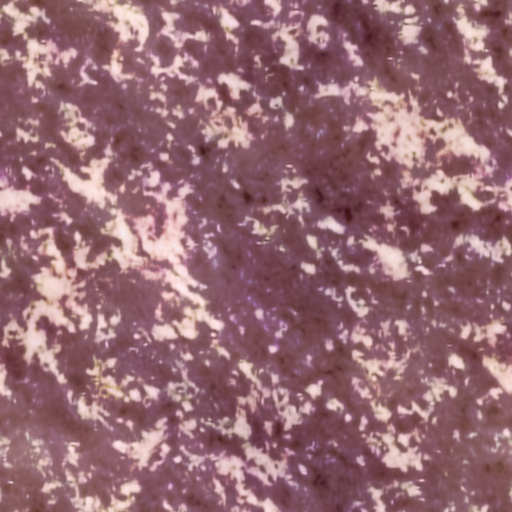
\includegraphics[scale=.32]{5/report/steerable/2_c.png}
      \caption{Generated}
    \end{center}
    \endminipage
    %
    \end{figure} 

    \begin{figure}[!htb]
    %
    \minipage{0.5\textwidth}
    \begin{center}
      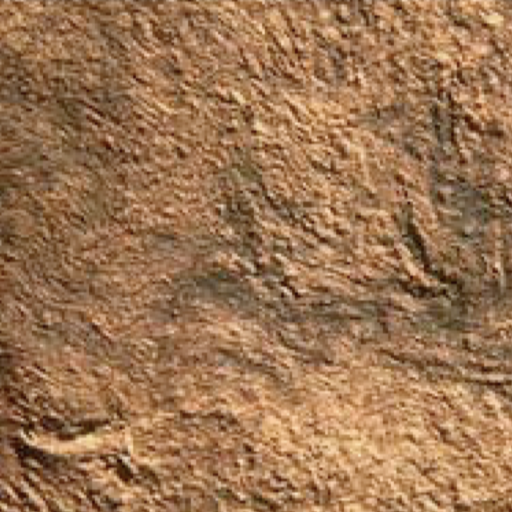
\includegraphics[scale=.32]{5/report/steerable/3.png}
      \caption{Original}
    \end{center}
    \endminipage \hfill
    %
    \minipage{0.5\textwidth}
    \begin{center}
      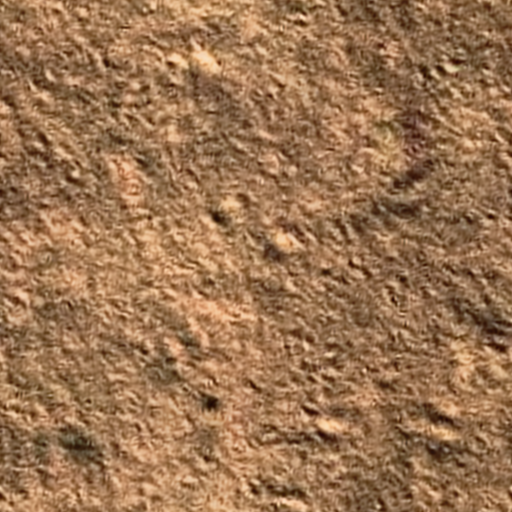
\includegraphics[scale=.32]{5/report/steerable/3_c.png}
      \caption{Generated}
    \end{center}
    \endminipage
    %
    \end{figure} 
% -------------------------------------------------------
\pagebreak\\

    \begin{figure}[!htb]
    %
    \minipage{0.5\textwidth}
    \begin{center}
      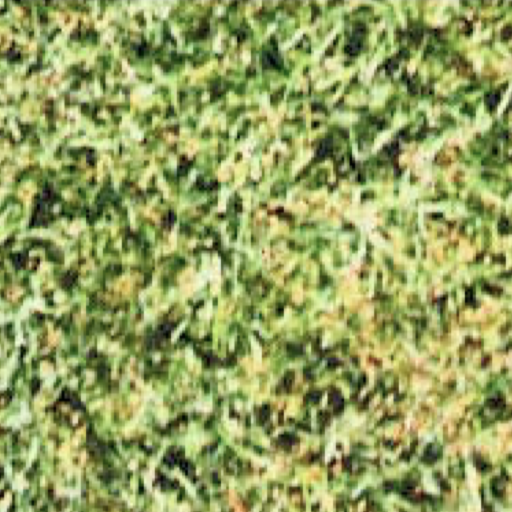
\includegraphics[scale=.34]{5/report/steerable/9.png}
      \caption{Original}
    \end{center}
    \endminipage \hfill
    %
    \minipage{0.5\textwidth}
    \begin{center}
      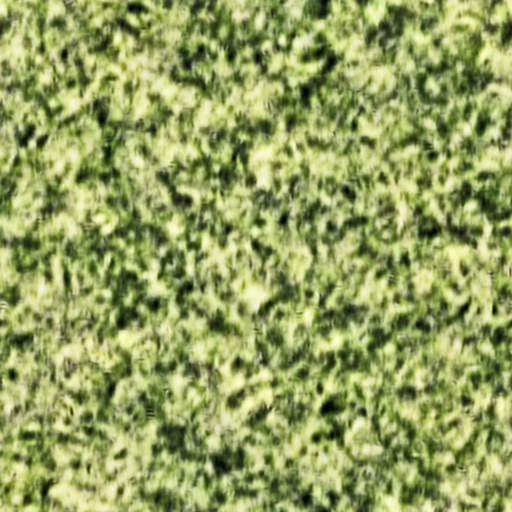
\includegraphics[scale=.34]{5/report/steerable/9_c.png}
      \caption{Generated}
    \end{center}
    \endminipage
    %
    \end{figure} 

    \begin{figure}[!htb]
    %
    \minipage{0.5\textwidth}
    \begin{center}
      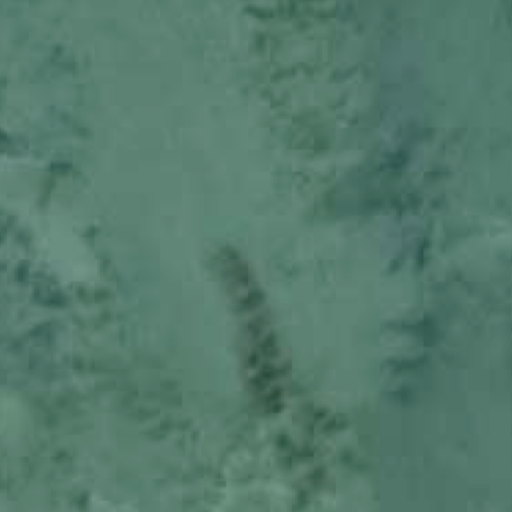
\includegraphics[scale=.34]{5/report/steerable/5.png}
      \caption{Original}
    \end{center}
    \endminipage \hfill
    %
    \minipage{0.5\textwidth}
    \begin{center}
      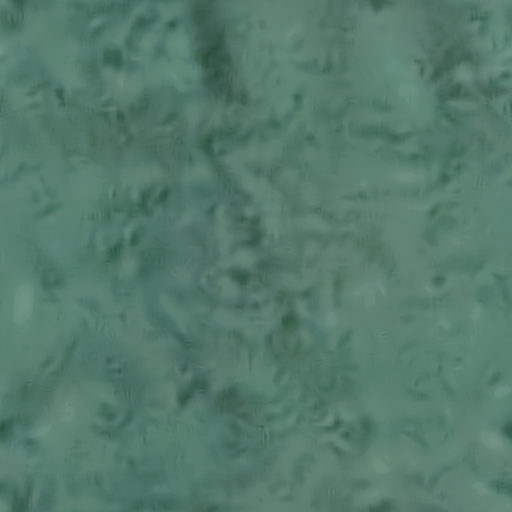
\includegraphics[scale=.34]{5/report/steerable/5_c.png}
      \caption{Generated}
    \end{center}
    \endminipage
    %
    \end{figure} 

    \begin{figure}[!htb]
    %
    \minipage{0.5\textwidth}
    \begin{center}
      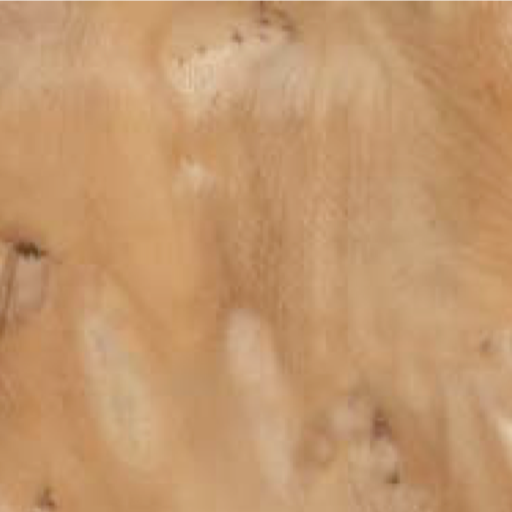
\includegraphics[scale=.34]{5/report/steerable/7.png}
      \caption{Original}
    \end{center}
    \endminipage \hfill
    %
    \minipage{0.5\textwidth}
    \begin{center}
      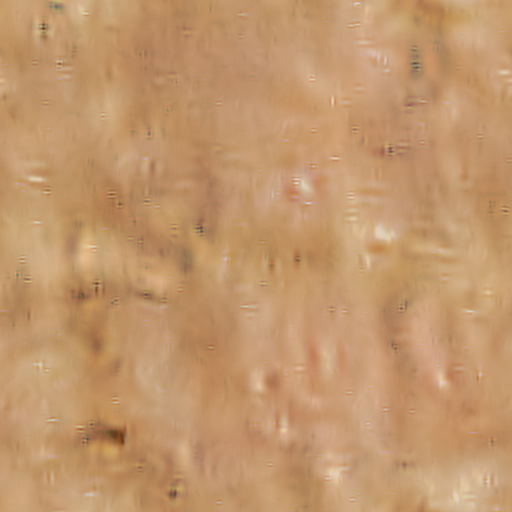
\includegraphics[scale=.34]{5/report/steerable/7_c.png}
      \caption{Generated}
    \end{center}
    \endminipage
    %
    \end{figure} 
% -------------------------------------------------------
\pagebreak\\

    \begin{figure}[!htb]
    %
    \minipage{0.5\textwidth}
    \begin{center}
      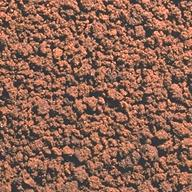
\includegraphics[scale=.34]{5/report/steerable/14.png}
      \caption{Original}
    \end{center}
    \endminipage \hfill
    %
    \minipage{0.5\textwidth}
    \begin{center}
      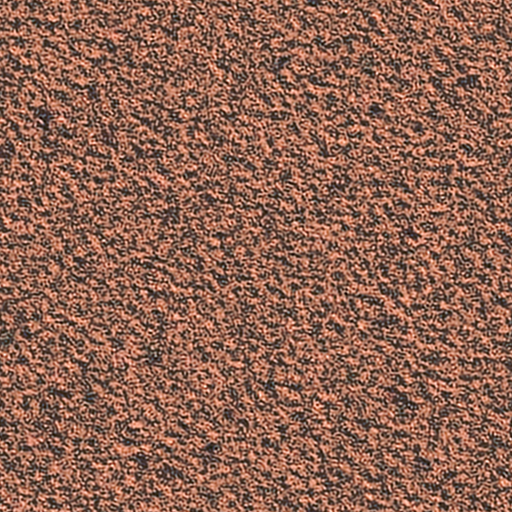
\includegraphics[scale=.34]{5/report/steerable/14_c.png}
      \caption{Generated}
    \end{center}
    \endminipage
    %
    \end{figure} 

    \begin{figure}[!htb]
    %
    \minipage{0.5\textwidth}
    \begin{center}
      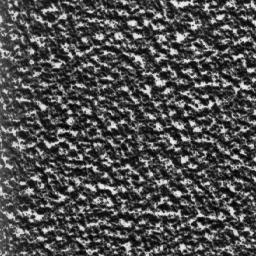
\includegraphics[scale=.32]{5/report/steerable/13.png}
      \caption{Original}
    \end{center}
    \endminipage \hfill
    %
    \minipage{0.5\textwidth}
    \begin{center}
      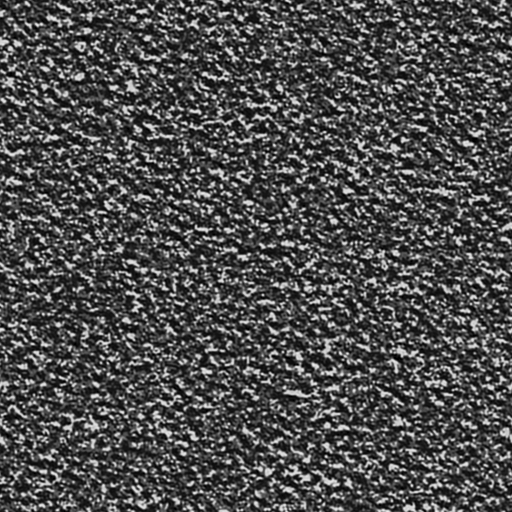
\includegraphics[scale=.34]{5/report/steerable/13_c.png}
      \caption{Generated}
    \end{center}
    \endminipage
    %
    \end{figure} 

    \begin{figure}[!htb]
    %
    \minipage{0.5\textwidth}
    \begin{center}
      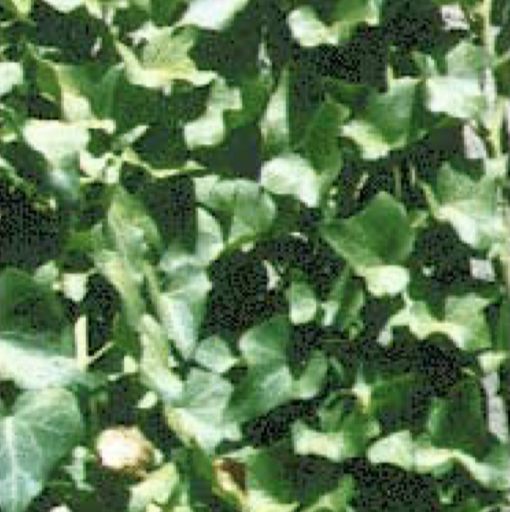
\includegraphics[scale=.14]{5/report/steerable/4.png}
      \caption{Original}
    \end{center}
    \endminipage \hfill
    %
    \minipage{0.5\textwidth}
    \begin{center}
      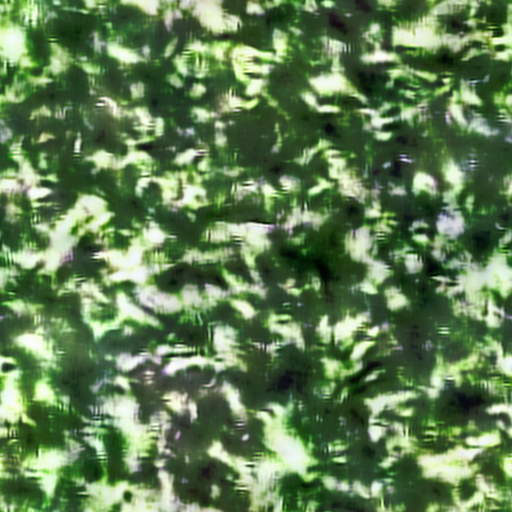
\includegraphics[scale=.34]{5/report/steerable/4_c.png}
      \caption{Generated}
    \end{center}
    \endminipage
    %
    \end{figure} 
% ------------------------------------------------------- 
\pagebreak
The steerable pyramid method works great in many scenarios, giving us very good approximate of textures. But, it fails very bad in case of sharp edges and more-constrained structures, as given below...\\

    \begin{figure}[!htb]
    %
    \minipage{0.5\textwidth}
    \begin{center}
      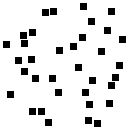
\includegraphics[scale=.3]{5/report/steerable/16.png}
      \caption{Original}
    \end{center}
    \endminipage \hfill
    %
    \minipage{0.5\textwidth}
    \begin{center}
      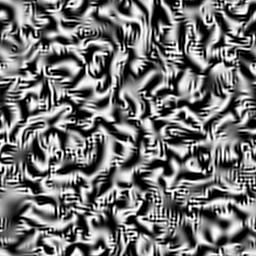
\includegraphics[scale=.3]{5/report/steerable/16_c.png}
      \caption{Generated}
    \end{center}
    \endminipage
    %
    \end{figure} 

    \begin{figure}[!htb]
    %
    \minipage{0.5\textwidth}
    \begin{center}
      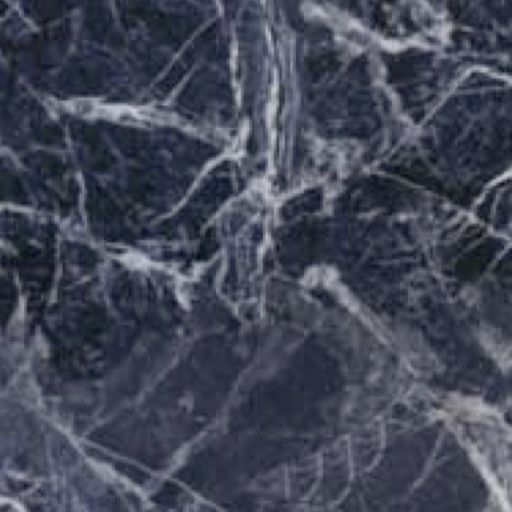
\includegraphics[scale=.32]{5/report/steerable/11.png}
      \caption{Original}
    \end{center}
    \endminipage \hfill
    %
    \minipage{0.5\textwidth}
    \begin{center}
      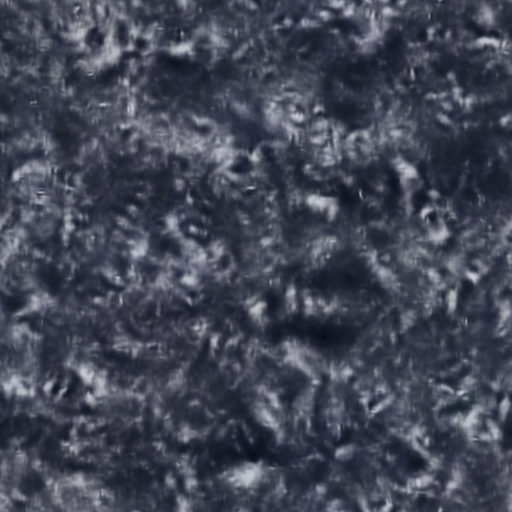
\includegraphics[scale=.34]{5/report/steerable/11_c.png}
      \caption{Generated}
    \end{center}
    \endminipage
    %
    \end{figure} 

    \begin{figure}[!htb]
    %
    \minipage{0.5\textwidth}
    \begin{center}
      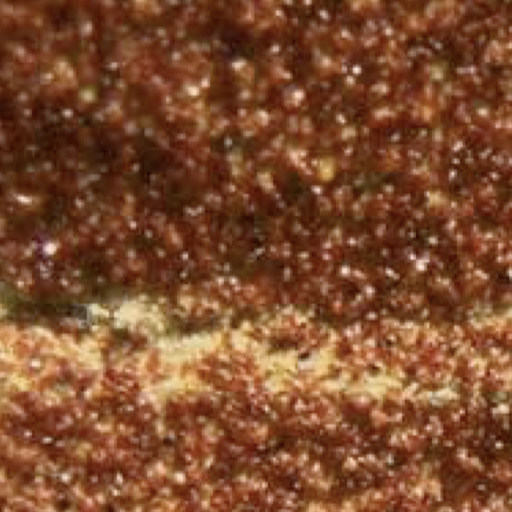
\includegraphics[scale=.34]{5/report/steerable/12.png}
      \caption{Original}
    \end{center}
    \endminipage \hfill
    %
    \minipage{0.5\textwidth}
    \begin{center}
      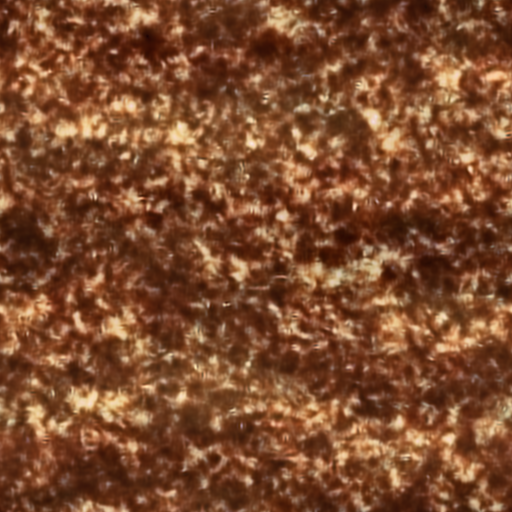
\includegraphics[scale=.34]{5/report/steerable/12_c.png}
      \caption{Generated}
    \end{center}
    \endminipage
    %
    \end{figure} 
% ------------------------------------------------------- 
% ------------------------------------------------------- 
    \pagebreak
% -------------------------------------------------------
% Character Detection
    \subsection*{Non Parametric Synthesis (Bonus)}
    This method exploits the fact that textures are locally repetitive, and thus allowing neighbourhood matching get the ideal extensions to boundary pixels.\\
    I have picked a generic 2D matrix to represent my neighbourhood (depending on vertical/horizontal extension).\\
    Now, to extend an image, I just fill the image horizontally and then extend it vertically downwards.\\
    Since, no apt optimisations were performed the process was very compute intensive and time consuming.\\
    Results were very promising and are presented below.\\

    \begin{figure}[!htb]
    %
    \minipage{0.4\textwidth}
    \begin{center}
      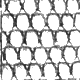
\includegraphics[scale=.6]{5/report/non_parametric/1.png}
      \caption{Original}
    \end{center}
    \endminipage
    %
    \minipage{0.5\textwidth}
    \begin{center}
      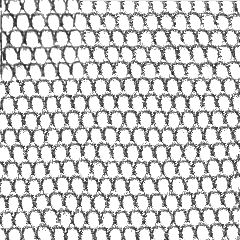
\includegraphics[scale=1.0]{5/report/non_parametric/1_created.png}
      \caption{Generated}
    \end{center}
    \endminipage
    %
    \end{figure} 
% -------------------------------------------------------

% -------------------------------------------------------
\pagebreak \\

    \begin{figure}[!htb]
    %
    \minipage{0.4\textwidth}
    \begin{center}
      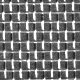
\includegraphics[scale=.6]{5/report/non_parametric/2.png}
      \caption{Original}
    \end{center}
    \endminipage
    %
    \minipage{0.5\textwidth}
    \begin{center}
      \includegraphics[scale=1.0]{5/report/non_parametric/2_created.png}
      \caption{Generated}
    \end{center}
    \endminipage
    %
    \end{figure}

    \begin{figure}[!htb]
    %
    \minipage{0.4\textwidth}
    \begin{center}
      \includegraphics[scale=.6]{5/report/non_parametric/3.png}
      \caption{Original}
    \end{center}
    \endminipage
    %
    \minipage{0.5\textwidth}
    \begin{center}
      \includegraphics[scale=1.0]{5/report/non_parametric/3_created.png}
      \caption{Generated}
    \end{center}
    \endminipage
    %
    \end{figure}
% -------------------------------------------------------
\pagebreak \\

    \begin{figure}[!htb]
    %
    \minipage{0.4\textwidth}
    \begin{center}
      \includegraphics[scale=.6]{5/report/non_parametric/4.png}
      \caption{Original}
    \end{center}
    \endminipage
    %
    \minipage{0.5\textwidth}
    \begin{center}
      \includegraphics[scale=1.0]{5/report/non_parametric/4_created.png}
      \caption{Generated}
    \end{center}
    \endminipage
    %
    \end{figure}
    
The results (so far) work very well with almost any filter size, since the feature repetition is periodic. Whereas, such is not always the case and a poor filter choice might lead to a structurally correct yet irrelevant image. Consider below for instance.\\[5pt]

    \begin{figure}[!htb]
    %
    \minipage{0.4\textwidth}
    \begin{center}
      \includegraphics[scale=.6]{5/report/non_parametric/5.png}
      \caption{Original}
    \end{center}
    \endminipage
    %
    \minipage{0.5\textwidth}
    \begin{center}
      \includegraphics[scale=1.0]{5/report/non_parametric/5_created.png}
      \caption{Generated}
    \end{center}
    \endminipage
    %
    \end{figure}
%--------------------------------------------- 
\pagebreak
%---------------------------------------------
% Summary
\subsection*{Summary}
    This assignment was very interesting, and I learnt a lot of new things.\\
    Covering all the aspects of texture recognition, I feel very confident in the idea and its relevance. I'd love to pursue it further as well. I am grateful for having been introduced to such an interesting topic.\\
    What was discussed in class was very helpful and useful. \\
    Thanks and Regards\\
    Rajbir
\end{document}